\documentclass[11pt,a4paper]{article}

\usepackage[utf8]{inputenc}
\usepackage[margin=1in]{geometry}
\usepackage{amsmath,amssymb,amsfonts}
\usepackage{graphicx}
\usepackage{booktabs}
\usepackage{array}
\usepackage{tabularx}
\usepackage{tikz}
\usetikzlibrary{shapes.geometric, arrows.meta, positioning}
\usepackage{pgfplots}
\pgfplotsset{compat=1.18}
\usepackage{cite}
\usepackage{hyperref}
\usepackage{authblk}
\usepackage{xcolor}

\hypersetup{
    colorlinks=true,
    linkcolor=black,
    citecolor=blue,
    urlcolor=blue
}

\title{\textbf{MEDICORE: An Intelligent Blockchain-Based Framework for Pharmaceutical Supply Chain Traceability, Verification, and Anomaly Monitoring}}

\author[1]{Aditya Kumar Roy\thanks{Corresponding author. E-mail: \texttt{2301020723@cgu-odisha.ac.in}}}
\author[1]{Krishna Das}

\affil[1]{Department of Computer Science and Engineering, C. V. Raman Global University, Bhubaneswar, Odisha, 752054, India}

\date{}

\begin{document}

\maketitle

\begin{abstract}
Pharmaceutical supply chains require reliable traceability, controlled transfer of ownership, product verification, quality monitoring, and rapid response to recalls and abnormal supply-chain events. Conventional systems frequently distribute these functions across organizational boundaries, creating challenges in maintaining consistent records and obtaining an end-to-end view of product movement. This paper presents MEDICORE, a blockchain-based pharmaceutical supply-chain framework designed to integrate entity identity, batch management, quality approval, shipment tracking, QR-based verification, recall management, cold-chain monitoring, and anomaly identification within a unified system. MEDICORE uses Solidity smart contracts deployed on an Ethereum-compatible blockchain for authorization-sensitive and traceability-critical operations, while operational telemetry and high-volume information are maintained through an off-chain database. The framework introduces permanent entity identifiers, digital product passports, quantity-conservation constraints, shipment verification codes, role-based access control, GPS monitoring, temperature monitoring, and explainable supply-chain risk indicators. QR codes provide access to a verifiable digital product record without requiring a consumer wallet.

The system is evaluated using the implemented prototype dataset, automated contract tests, and a local EVM benchmark covering batch minting, quality approval, shipment creation, cryptographic receipt, and public QR reading. Dataset-derived quantities and verification scenarios are reported separately from performance measurements so that prototype state is not confused with repeated statistical experiments. The current prototype also identifies practical limitations related to continuous IoT sensing, document storage, customer integration, backend authentication, and automated testing. The resulting framework demonstrates how blockchain and intelligent monitoring mechanisms can be combined to improve pharmaceutical supply-chain visibility and auditability while maintaining a clear distinction between digital record verification and physical product authenticity.
\end{abstract}

\noindent\textbf{Keywords:} Blockchain, Pharmaceutical Supply Chain, Drug Traceability, Smart Contracts, Digital Product Passport, QR Verification, Cold Chain, GPS Monitoring, Anomaly Detection, Supply Chain Intelligence

\vspace{1.5em}

\section{Introduction}
The pharmaceutical supply chain involves multiple independent entities, including manufacturers, wholesalers, logistics providers, pharmacies, quality officers, regulators, and customers. A pharmaceutical product may pass through several ownership and custody transitions before reaching the patient. Maintaining reliable records across these transitions is essential for product traceability, quality assurance, recall management, and regulatory compliance.

Traditional pharmaceutical supply-chain information systems commonly depend on centralized databases and organization-specific records. Such architectures can make cross-organizational verification difficult because participants may maintain separate records with different access controls, update mechanisms, and levels of visibility. When a product needs to be traced across multiple organizations, information must often be reconstructed from several systems.

Blockchain technology provides a distributed ledger in which authorized participants can record transactions and events in a tamper-evident manner. Smart contracts can additionally enforce predefined authorization and state-transition rules. Previous research has explored blockchain-based pharmaceutical tracking and tracing systems, demonstrating the applicability of distributed ledgers to pharmaceutical supply chains \cite{liu2021blockchain,hosseini2021blockchain}.

However, blockchain alone does not solve all pharmaceutical supply-chain problems. Physical product conditions, transportation routes, temperature, organizational credentials, and operational events originate outside the blockchain. Consequently, a practical system requires a hybrid architecture combining blockchain records with off-chain databases, document storage, location information, sensor telemetry, and verification interfaces.

This work presents MEDICORE, a prototype framework that combines blockchain-based traceability with supply-chain monitoring and anomaly identification. The framework focuses on five major objectives:
\begin{enumerate}
    \item Establishing persistent digital identities for supply-chain participants.
    \item Maintaining blockchain-backed pharmaceutical batch and transfer records.
    \item Providing QR-based digital product and shipment verification.
    \item Monitoring shipment location and cold-chain conditions.
    \item Identifying supply-chain anomalies that may require investigation.
\end{enumerate}

The principal contributions of this work are:
\begin{itemize}
    \item A role-controlled blockchain framework for pharmaceutical supply-chain operations.
    \item A permanent entity identity model connecting participants, facilities, licenses, batches, shipments, and audit records.
    \item A digital product passport and QR verification mechanism for accessing pharmaceutical supply-chain records.
    \item A quantity-conservation mechanism that prevents unauthorized creation of additional transferable inventory within the recorded system.
    \item Integration of shipment, GPS, temperature, recall, and investigation information into a unified monitoring framework.
    \item An explainable anomaly-monitoring layer that produces risk signals rather than treating anomalies as proof of fraud.
    \item An experimental methodology for evaluating authorization, traceability, verification, monitoring, and system performance.
\end{itemize}

\section{Related Work}
Blockchain technology has been investigated as a mechanism for improving traceability and transparency in pharmaceutical supply chains, with broader supply-chain studies highlighting provenance, multi-party coordination, and tamper-evident event histories \cite{nakamoto2008bitcoin,szabo1997formalizing,crosby2016blockchain,casino2019systematic,kamilaris2019rise,saberi2019blockchain,queiroz2020blockchain,wang2019understanding}. Liu et al. proposed a blockchain-based smart tracking and tracing platform for pharmaceutical products, demonstrating how distributed ledger mechanisms can support supply-chain visibility \cite{liu2021blockchain}.

IoT-enabled monitoring adds a physical-observation layer to blockchain traceability; recent work emphasizes sensor integrity, cold-chain monitoring, and the need to treat anomalous readings as evidence requiring validation rather than proof of physical damage \cite{yadav2022blockchain,antal2018blockchain,mutambik2026blockchain,securitythreats2026}. Pharmaceutical cold chains introduce an additional requirement because medicines and vaccines may depend on controlled temperature conditions during transportation and storage. Hosseini Bamakan et al. examined blockchain-enabled pharmaceutical cold chains and discussed applications, challenges, and future directions \cite{hosseini2021blockchain}.

Recent studies have also investigated blockchain-based pharmaceutical supply-chain architectures using permissioned blockchain platforms and resource-aware implementations. TrackChain, for example, explored a Hyperledger-based pharmaceutical supply-chain architecture with emphasis on resource utilization \cite{nagasudha2024trackchain}.

Broader reviews of blockchain applications in pharmaceutical supply chains indicate that blockchain can support transparency, provenance, and controlled information sharing, while also presenting challenges related to interoperability, scalability, data quality, and integration with physical-world systems \cite{akram2024blockchain}.

Interoperability and serialization are also important for production deployment. GS1 EPCIS provides a standardized event vocabulary for what, when, where, why, sensor data, and certification information \cite{gs12024epcis,gs12024healthcare,gs12017global}. Recent 2025--2026 studies extend this direction toward scalable Ethereum and Layer-2 designs, blockchain--IPFS traceability, IoT anti-counterfeit monitoring, privacy-preserving recall, and blockchain--IoT--AI integration \cite{dutta2026blockchain,hasan2026blockchain,rajak2026scalable,drugtrace2026,zk2026privacy,devi2025blockchain,siyal2026traceability}. Product authentication is another related research direction. Blockchain can provide tamper-evident records associated with products, although authentication of the physical product remains dependent on the relationship between the digital identifier and the physical item \cite{henrichs2025quantum}.

MEDICORE differs from a purely ledger-centric approach by combining blockchain traceability with entity identity, shipment verification, QR access, GPS monitoring, cold-chain monitoring, recall propagation, and anomaly indicators in a single prototype architecture.

\section{Problem Formulation and Research Questions}
Let a pharmaceutical batch be represented as:
\begin{equation}
B = (I, P, M, Q, E, S)
\end{equation}
where:
\begin{itemize}
    \item $I$ is the batch identifier,
    \item $P$ is the product information,
    \item $M$ is the manufacturer,
    \item $Q$ is the initial quantity,
    \item $E$ is the expiry information,
    \item $S$ is the current lifecycle state.
\end{itemize}

A transfer is represented as:
\begin{equation}
T_i = (B, E_s, E_r, Q_i, S_i, t_i)
\end{equation}
where $E_s$ is the sender, $E_r$ is the receiver, $Q_i$ is the transferred quantity, $S_i$ is the shipment identifier, and $t_i$ is the transfer timestamp.

The quantity-conservation requirement is:
\begin{equation}
Q_{\text{initial}} = Q_{\text{remaining}} + \sum_{i=1}^n Q_i
\end{equation}

A transfer must therefore satisfy:
\begin{equation}
Q_{\text{transfer}} \le Q_{\text{available}}
\end{equation}

The research investigates the following questions:
\begin{enumerate}
    \item \textbf{RQ1:} Can blockchain-based role authorization restrict pharmaceutical supply-chain operations to authorized entities?
    \item \textbf{RQ2:} Can quantity-conservation rules maintain consistency between initial, transferred, and remaining batch quantities?
    \item \textbf{RQ3:} Can QR-based verification provide accessible verification of blockchain-backed pharmaceutical records?
    \item \textbf{RQ4:} Can GPS and temperature monitoring identify supply-chain events requiring investigation?
    \item \textbf{RQ5:} Can recall events propagate consistently through the digital supply-chain representation?
    \item \textbf{RQ6:} What are the transaction and operational performance characteristics of the implemented prototype?
\end{enumerate}

\section{MEDICORE Framework}
MEDICORE follows a hybrid architecture consisting of a React/Vite web application, Solidity smart contracts, a Node.js/Express operational backend, a SQLite telemetry database, QR interfaces, document references, and shipment-monitoring services. The implementation separates blockchain state transitions from high-frequency operational telemetry so that continuously changing GPS and sensor observations do not need to be written to the ledger.

\subsection{System Architecture}
The high-level architecture is illustrated conceptually in Fig.~\ref{fig:arch}.

\begin{figure}[htbp]
\centering
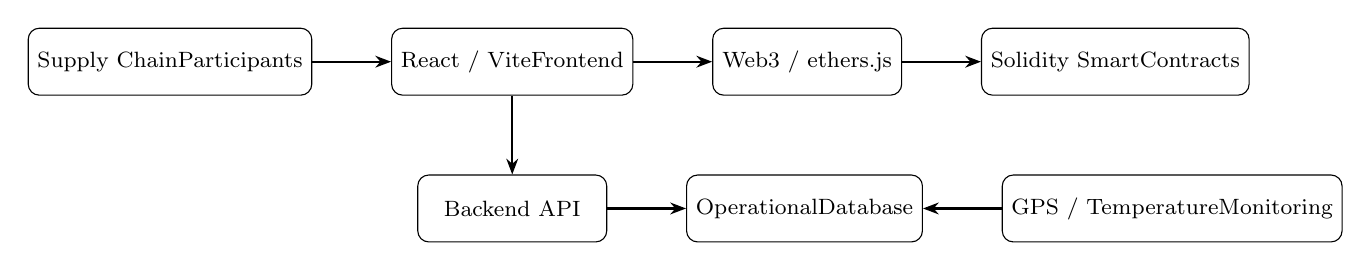
\begin{tikzpicture}[
    box/.style={rectangle, draw=black, rounded corners, minimum width=2.4cm, minimum height=0.85cm, text centered, font=\footnotesize},
    arrow/.style={-{Stealth[length=2mm]}, thick}
]
\node[box] (part) {Supply Chain\\Participants};
\node[box, right=1.0cm of part] (ui) {React / Vite\\Frontend};
\node[box, right=1.0cm of ui] (web3) {Web3 / ethers.js};
\node[box, right=1.0cm of web3] (sc) {Solidity Smart\\Contracts};

\node[box, below=1.0cm of ui] (api) {Backend API};
\node[box, right=1.0cm of api] (db) {Operational\\Database};
\node[box, right=1.0cm of db] (iot) {GPS / Temperature\\Monitoring};

\draw[arrow] (part) -- (ui);
\draw[arrow] (ui) -- (web3);
\draw[arrow] (web3) -- (sc);
\draw[arrow] (ui) -- (api);
\draw[arrow] (api) -- (db);
\draw[arrow] (iot) -- (db);
\end{tikzpicture}
\caption{Conceptual architecture of the MEDICORE framework.}
\label{fig:arch}
\end{figure}

The blockchain stores role authorization, batch creation, custody transitions, quantity constraints, cryptographic handoff commitments, recall decisions, entity status changes, and other traceability-critical events. The off-chain Node.js/Express and SQLite layer stores operational telemetry and anomaly observations, including GPS records and QR verification attempts. The React/Vite interface presents these sources through role-specific workspaces, Leaflet maps, and telemetry visualizations.

\subsection{Supply-Chain Roles}
The framework defines the following principal roles:

\begin{table}[htbp]
\centering
\caption{Principal MEDICORE supply-chain roles}
\label{tab:roles}
\vspace{0.5em}
\begin{tabularx}{\textwidth}{lX}
\toprule
\textbf{Role} & \textbf{Principal responsibilities} \\
\midrule
Manufacturer & Create batches, submit quality information, initiate distribution and shipments. \\
Wholesaler & Receive, verify, store, and distribute pharmaceutical products. \\
Transporter & Execute shipments and provide location information. \\
Pharmacy & Receive verified products and manage dispensing inventory. \\
Quality Officer & Review quality records and approve or investigate batches. \\
Regulator & Monitor incidents, recalls, entities, and supply-chain compliance. \\
Customer & Verify pharmaceutical product information through public verification. \\
Administrator & Manage entities, permissions, suspension, reinstatement, and audit operations. \\
\bottomrule
\end{tabularx}
\end{table}

\section{Blockchain and Smart Contract Design}
The blockchain layer implements authorization and state-transition logic using Solidity smart contracts.

\subsection{Entity Management}
Every registered participant is assigned a permanent entity identifier. The entity identifier is logically separated from the participant's wallet address. This distinction allows an entity to retain its identity when operational information changes, such as a wallet address, facility, or license.

An entity may have one of several states:
\begin{equation}
\text{Status} \in \{\text{ACTIVE}, \text{PENDING}, \text{SUSPENDED}, \text{UNDER\_INVESTIGATION}, \text{REINSTATED}\}
\end{equation}
Administrative actions are recorded as blockchain events and corresponding audit records.

\subsection{Batch Lifecycle}
A pharmaceutical batch passes through a controlled lifecycle:
\begin{equation}
\text{CREATED} \to \text{QUALITY\_PENDING} \to \text{QUALITY\_APPROVED} \to \text{AVAILABLE} \to \text{IN\_TRANSIT} \to \text{DELIVERED} \to \text{SOLD}
\end{equation}
Exception states include:
\begin{equation}
\text{FLAGGED}, \text{QUARANTINED}, \text{UNDER\_INVESTIGATION}, \text{RELEASED}, \text{RECALLED}, \text{EXPIRED}
\end{equation}
The state machine prevents operations that are inconsistent with the current batch state.

\subsection{Quantity Conservation}
A central design property is quantity conservation. For a batch with initial quantity $Q_0$:
\begin{equation}
Q_0 = Q_r + \sum_{i=1}^n Q_i
\end{equation}
where $Q_r$ is the remaining quantity and $Q_i$ represents each valid transfer. A transaction attempting:
\begin{equation}
Q_i > Q_r
\end{equation}
must be rejected. This mechanism reduces the possibility of creating additional transferable inventory through unauthorized application-level operations.

\subsection{Administrative Suspension}
Administrators can suspend registered entities when appropriate. A suspension record contains:
\begin{equation}
A = (E, R, X, C, W, t)
\end{equation}
where $E = \text{entity identifier}$, $R = \text{suspension reason}$, $X = \text{explanation}$, $C = \text{evidence reference}$, $W = \text{administrator wallet}$, and $t = \text{timestamp}$. Historical transactions remain preserved after suspension.

\section{Digital Product Passport and QR Verification}
MEDICORE associates each pharmaceutical batch with a digital product passport containing structured product and supply-chain information:
\begin{itemize}
    \item Product name.
    \item Batch identifier.
    \item Manufacturer.
    \item Manufacturing information.
    \item Expiry information.
    \item Quality status.
    \item Ownership history.
    \item Shipment history.
    \item Recall status.
    \item Verification events.
\end{itemize}

The QR code does not store the entire product record. Instead, it provides an identifier or verification URL. The verification process is:
\begin{equation}
\text{QR} \to \text{Identify} \to \text{Retrieve} \to \text{Validate} \to \text{Display}
\end{equation}
For shipment handoff, MEDICORE uses a single-use delivery secret. If the secret is $C$, the contract stores the commitment $\mathcal{H} = \text{keccak256}(C)$, while the receiving party supplies $C$ during receipt. This is a hash-commitment/preimage verification mechanism; it is not claimed here as a formal zero-knowledge proof.

The verification engine checks: (1) Batch existence, (2) Manufacturer registration, (3) Quality status, (4) Recall status, (5) Expiry status, (6) Shipment state where applicable, and (7) Blockchain record consistency.

\begin{table}[htbp]
\centering
\caption{QR verification outcomes}
\label{tab:qr_outcomes}
\vspace{0.5em}
\begin{tabularx}{\textwidth}{lX}
\toprule
\textbf{Result} & \textbf{Meaning} \\
\midrule
\texttt{VERIFIED} & The associated digital record satisfies the configured verification conditions. \\
\texttt{WARNING} & The record exists but contains an issue requiring attention, such as a recall, temperature incident, or investigation. \\
\texttt{INVALID} & The identifier or associated record cannot be verified. \\
\bottomrule
\end{tabularx}
\end{table}

Importantly, QR verification validates the associated digital record. It does not independently establish the physical authenticity of the medicine.

\section{Supply-Chain Monitoring and Anomaly Detection}

\subsection{GPS Monitoring}
Shipment location is maintained separately from the blockchain. A location observation is represented as:
\begin{equation}
L_i = (S, \lambda, \phi, a, v, h, t)
\end{equation}
where $S = \text{shipment identifier}$, $\lambda = \text{latitude}$, $\phi = \text{longitude}$, $a = \text{positional accuracy}$, $v = \text{speed}$, $h = \text{heading}$, and $t = \text{timestamp}$. The origin is derived from the manufacturer's registered facility and the destination is derived from the receiving entity's facility.

\subsection{Cold-Chain Monitoring}
For a medicine requiring temperature range:
\begin{equation}
T_{\min} \le T(t) \le T_{\max}
\end{equation}
a reading outside the configured range generates a monitoring incident. For example, for a medicine requiring 2$^\circ$C--8$^\circ$C:
\begin{equation}
2 \le T(t) \le 8
\end{equation}
is considered within the configured monitoring range. A temperature excursion should be treated as a quality signal requiring investigation rather than automatically interpreted as proof of product damage.

\subsection{Anomaly Monitoring}
MEDICORE considers multiple operational signals: route deviations, impossible journeys, excessive transfer speed, unusual transfer quantities, repeated QR scans, duplicate verification attempts, suspended-entity activity, temperature excursions, recall violations, and quantity inconsistencies. A conceptual risk function is:
\begin{equation}
R = w_T A_T + w_G A_G + w_Q A_Q + w_V A_V + w_S A_S
\end{equation}
where $A_T = \text{temperature anomaly}$, $A_G = \text{geographic anomaly}$, $A_Q = \text{quantity anomaly}$, $A_V = \text{verification anomaly}$, $A_S = \text{status or suspension anomaly}$, and $w_i = \text{configured weights}$.

The prototype also implements a concrete QR-abuse sentinel: after three consecutive incorrect verification-code submissions for a shipment, the backend creates a \texttt{SUSPICIOUS\_QR} incident for regulator review. Route-deviation and telemetry-based signals are similarly treated as investigation indicators. The risk value is an anomaly indicator and not a direct determination of fraud or illegal activity.

\section{MEDICORE Project Visual Evidence}
The implemented MEDICORE prototype contains role-specific workspaces covering manufacturing, quality assurance, distribution, logistics, pharmacy operations, regulatory oversight, public verification, and system administration. Figures~\ref{fig:transporter}--\ref{fig:admin} present representative screenshots captured from the implemented system. These screenshots are included as implementation evidence rather than as independent experimental observations. Consequently, numerical values visible in a dashboard are not used to replace the controlled dataset and benchmark measurements reported in Sections~10 and 11.

\begin{figure}[htbp]
\centering
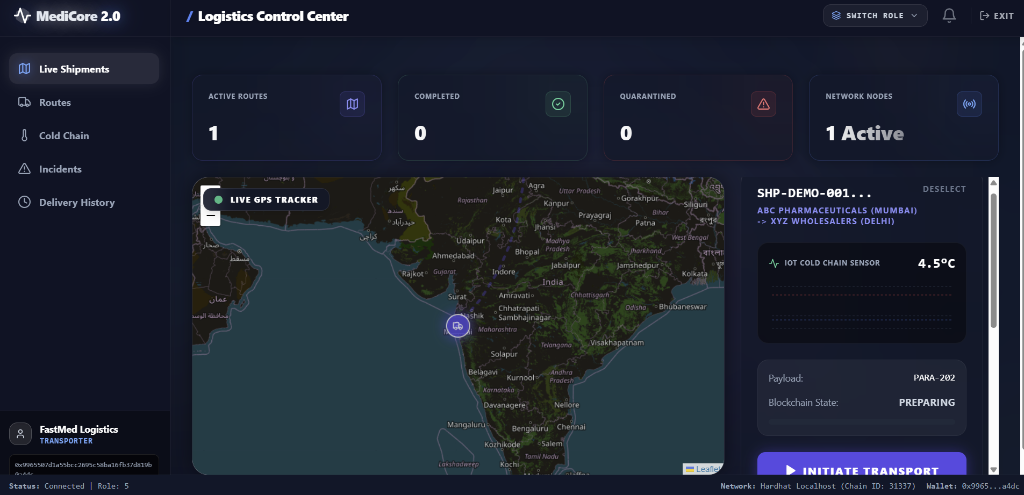
\includegraphics[width=0.88\textwidth]{fig2.png}
\caption{MEDICORE Transporter Logistics Control Center showing an active shipment, live GPS tracking, route context, cold-chain sensor reading, blockchain shipment state, and transport controls.}
\label{fig:transporter}
\end{figure}

The screenshots also demonstrate the hybrid nature of the platform. Operational views combine blockchain state with off-chain telemetry, maps, inventory records, verification interfaces, and role-specific controls. The public verification screen is intentionally read-only, whereas administrative and operational workspaces expose actions according to the connected role.

\section{Implementation}
MEDICORE was implemented as a web-based application using a React/Vite frontend and Solidity smart contracts.

\begin{figure}[htbp]
\centering
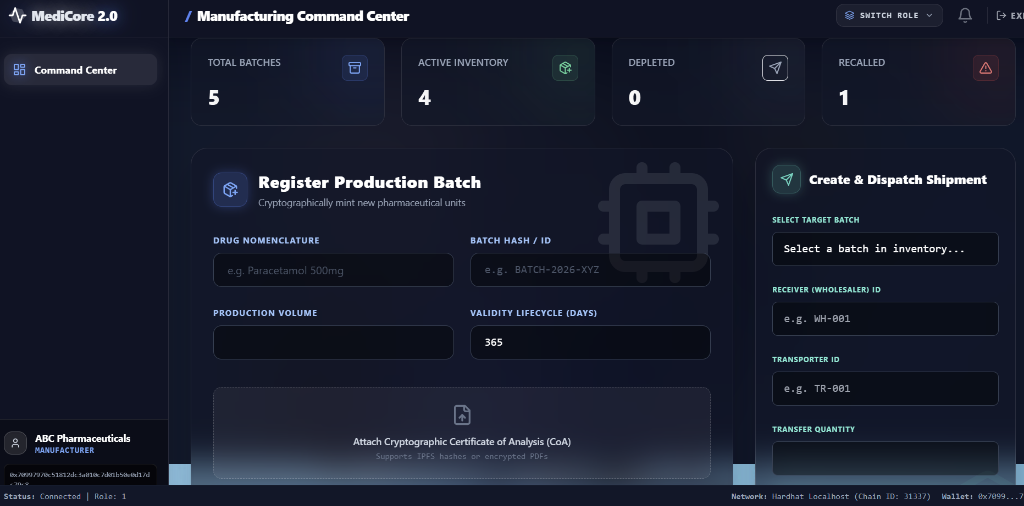
\includegraphics[width=0.88\textwidth]{fig3.png}
\caption{MEDICORE Manufacturing Command Center showing production-batch registration and shipment dispatch fields for a manufacturer.}
\label{fig:mfr}
\end{figure}

\begin{figure}[htbp]
\centering
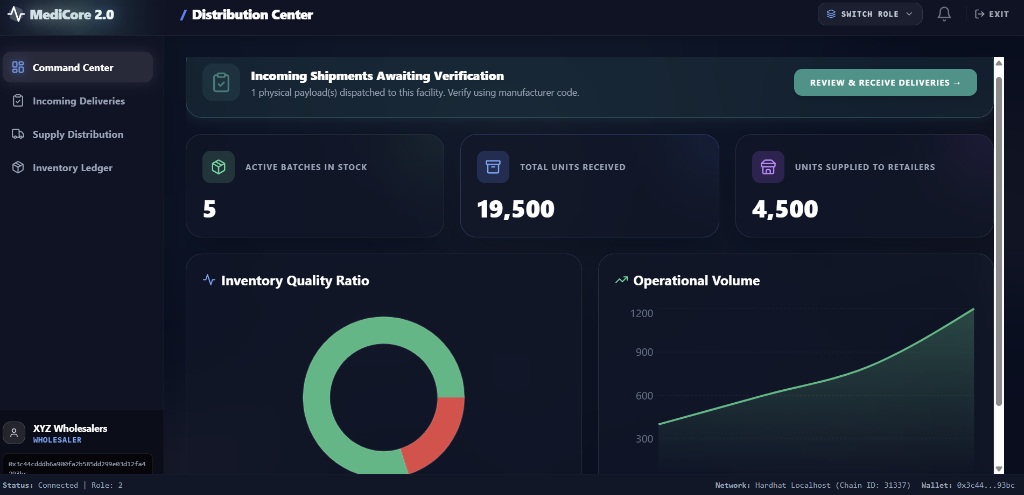
\includegraphics[width=0.88\textwidth]{fig4.png}
\caption{MEDICORE Wholesaler Distribution Center showing incoming-shipment verification, active inventory, received units, and distribution analytics.}
\label{fig:whl}
\end{figure}

\begin{figure}[htbp]
\centering
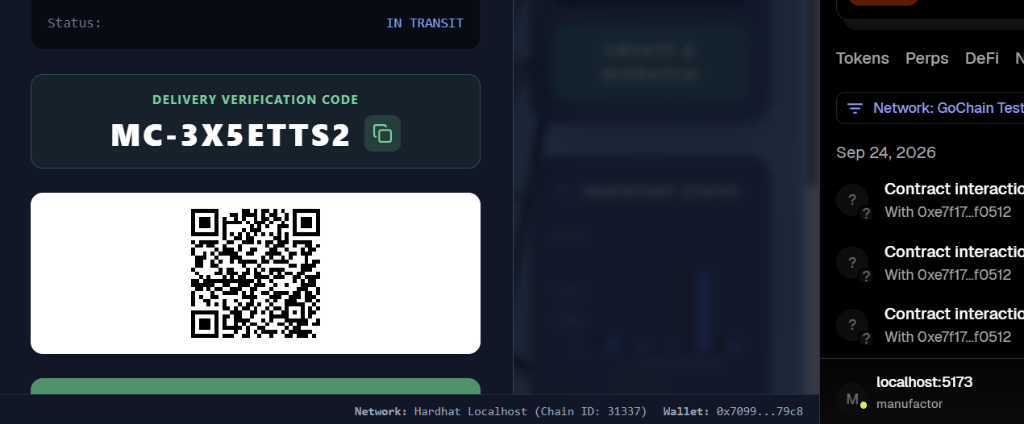
\includegraphics[width=0.75\textwidth]{fig5.png}
\caption{MEDICORE shipment handoff interface displaying a delivery verification code and QR representation. The code is used as the receiver-side preimage for the on-chain hash commitment.}
\label{fig:handoff_ui}
\end{figure}

The principal technologies include:

\begin{table}[htbp]
\centering
\caption{MEDICORE implementation technologies}
\label{tab:tech}
\vspace{0.5em}
\begin{tabularx}{\textwidth}{lX}
\toprule
\textbf{Component} & \textbf{Technology} \\
\midrule
Frontend & React 18, Vite, Tailwind CSS \\
Smart Contracts & Solidity \\
Blockchain Development & Hardhat \\
Blockchain Interaction & ethers.js and Web3 wallet integration \\
Backend & Node.js and Express \\
Operational Database & SQLite \\
Maps & Leaflet with OpenStreetMap-based mapping \\
Visualization & Recharts for telemetry and operational views \\
QR & Dynamic QR generation, scanning, and verification \\
Security Components & OpenZeppelin contract protections and role controls \\
Research Tooling & Python, Pandas, and Matplotlib for benchmark processing/plots \\
\bottomrule
\end{tabularx}
\end{table}

\subsection{Shipment Workflow}
The shipment workflow consists of:
\begin{enumerate}
    \item Manufacturer selects a quality-approved batch.
    \item Receiver and transporter are selected.
    \item Available quantity is validated against on-chain inventory.
    \item Origin and destination are resolved from registered facility information.
    \item Shipment is created and assigned a unique shipment reference.
    \item A single-use delivery secret is generated and its Keccak-256 commitment is associated with the shipment.
    \item A QR verification link provides access to shipment verification.
    \item Transport telemetry is collected through the operational backend.
    \item The receiving party supplies the delivery secret to complete the cryptographic receipt.
    \item The shipment state and custody record are updated after successful receipt.
\end{enumerate}

\begin{figure}[htbp]
\centering
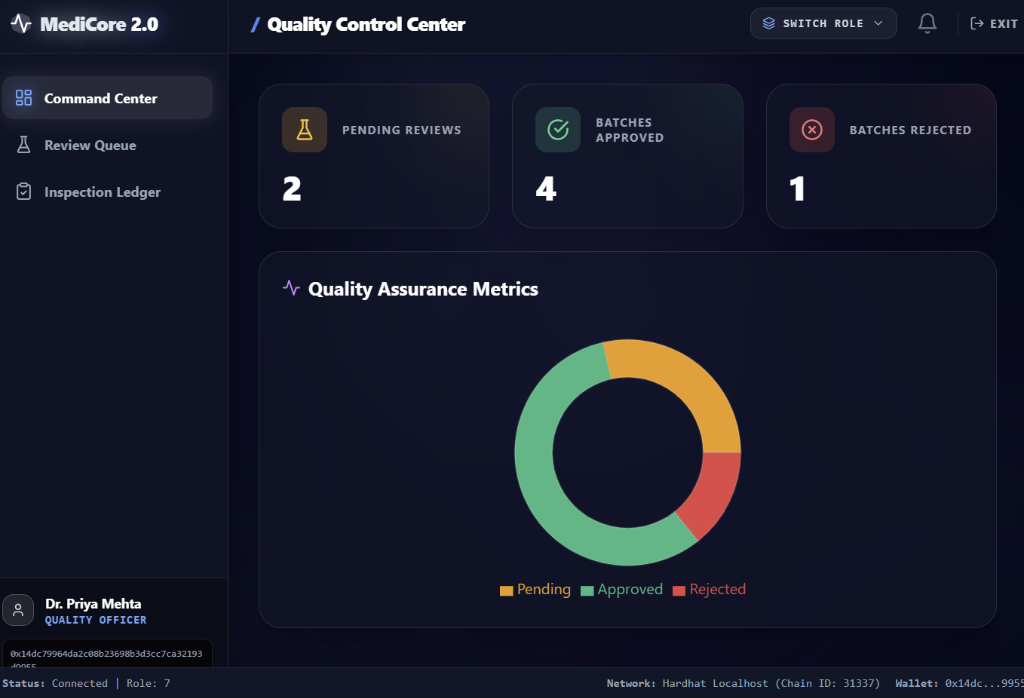
\includegraphics[width=0.88\textwidth]{fig6.png}
\caption{MEDICORE Quality Control Center showing pending reviews, approved batches, rejected batches, and quality-assurance metrics for the quality-officer role.}
\label{fig:quality_ui}
\end{figure}

\subsection{Recall Workflow}
The recall workflow consists of:
\begin{equation}
\text{REQUESTED} \to \text{UNDER\_REVIEW} \to \text{APPROVED} \to \text{ACTIVE} \to \text{COMPLETED}
\end{equation}
Once a recall is active, verification interfaces can identify the affected batch and communicate the recall status to users.

\section{Experimental Methodology}
The experimental evaluation is grounded in the actual MEDICORE prototype dataset rather than an externally generated pharmaceutical dataset. The current demonstration contains seven registered supply-chain entities, five pharmaceutical batches, eight recorded transfer transactions, three supporting documents, one active recall, and one recorded temperature violation. The evaluation distinguishes between values already present in the prototype and performance measurements that must be collected by repeated execution. No unmeasured latency, gas, accuracy, or anomaly-detection values are reported as experimental results.

\begin{figure}[htbp]
\centering
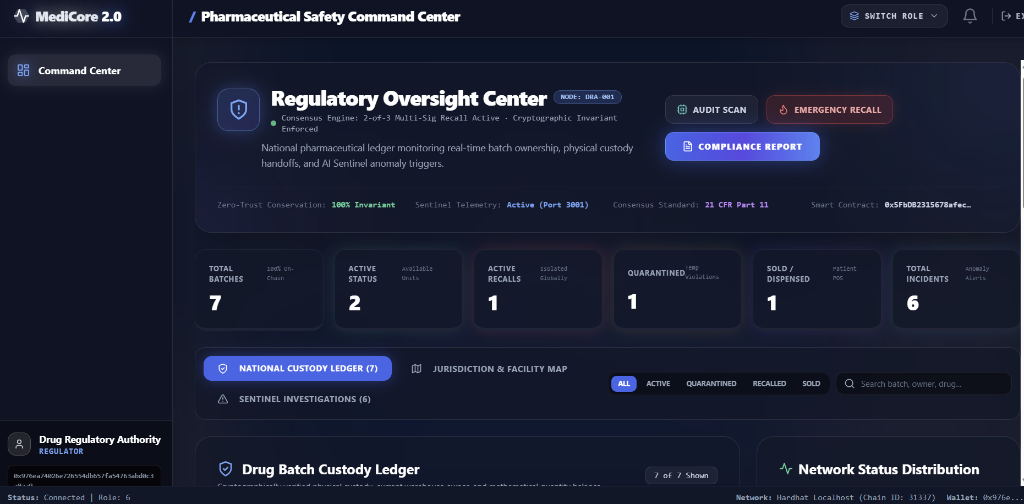
\includegraphics[width=0.88\textwidth]{fig7.png}
\caption{MEDICORE Pharmaceutical Safety Command Center showing regulatory oversight, custody-ledger access, recall and quarantine indicators, and Sentinel investigation monitoring.}
\label{fig:regulator_ui}
\end{figure}

\subsection{Experimental Environment}
MEDICORE is evaluated as an Ethereum-compatible blockchain application using Solidity smart contracts and the implemented web interface. Blockchain state is used for authorization-sensitive and traceability-critical operations, while the prototype also uses an off-chain database for operational telemetry and application data. GPS records are represented through the implemented shipment-monitoring workflow, and cold-chain observations are evaluated using the prototype's temperature-monitoring mechanism. The current cold-chain scenario is a controlled/simulated observation rather than a continuous physical IoT deployment.

\subsection{Prototype Dataset}
Table~\ref{tab:prototype_dataset} summarizes the data currently represented in the MEDICORE demonstration environment.

\subsection{Batch and Transfer Dataset}
The five batches and their currently recorded transfers are shown in Table~\ref{tab:batch_data}. The remaining quantity is derived directly from the initial quantity and the transfers recorded for the corresponding batch.

\begin{figure}[htbp]
\centering
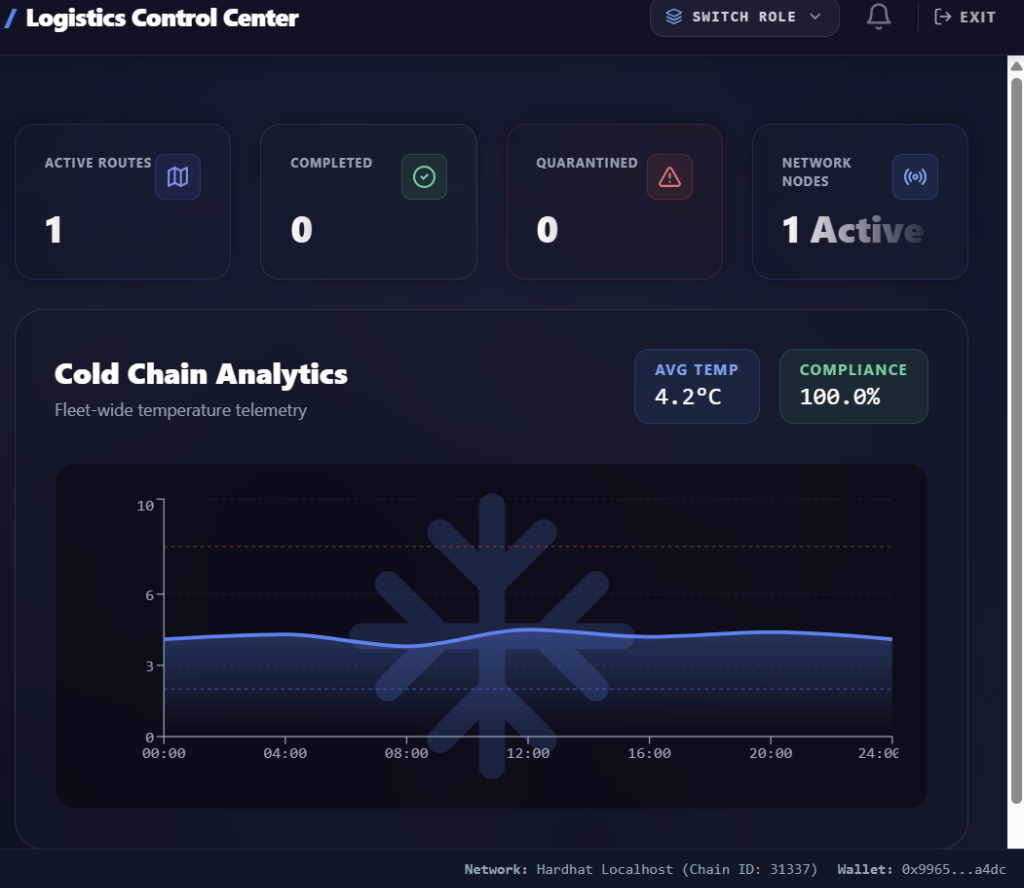
\includegraphics[width=0.88\textwidth]{fig8.png}
\caption{MEDICORE Cold Chain Analytics view showing fleet-wide temperature telemetry, average temperature, compliance percentage, and the monitored temperature curve.}
\label{fig:cold_chain_ui}
\end{figure}

\subsection{Quantity Conservation Experiment}
Quantity conservation is evaluated from the actual batch records. For each batch $b$, the recorded remaining quantity must equal the initial quantity minus all recorded outgoing transfers:
\begin{equation}
Q_{\text{rem}}(b) = Q_{\text{initial}}(b) - \sum_{i=1}^{n_b} Q_i(b)
\end{equation}
Equivalently,
\begin{equation}
Q_{\text{initial}}(b) = Q_{\text{rem}}(b) + \sum_{i=1}^{n_b} Q_i(b)
\end{equation}

For the current prototype data, the five conservation checks are:
\begin{align}
10,000 &= 4,450 + 4,000 + 1,500 + 50 \\
5,000 &= 3,000 + 2,000 \\
2,000 &= 1,500 + 500 \\
50,000 &= 37,000 + 10,000 + 3,000 \\
8,000 &= 5,000 + 3,000
\end{align}

\begin{figure}[htbp]
\centering
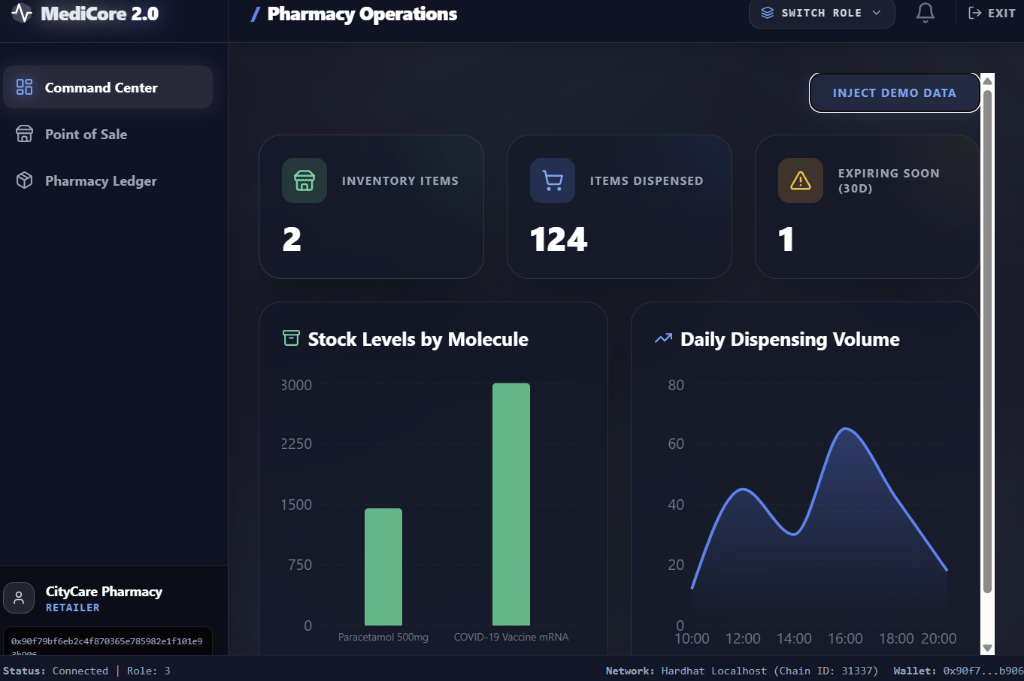
\includegraphics[width=0.88\textwidth]{fig9.png}
\caption{MEDICORE Pharmacy Operations workspace showing inventory items, dispensed items, expiry monitoring, stock levels by molecule, and daily dispensing volume.}
\label{fig:pharmacy_ui}
\end{figure}

All five equations balance for the currently recorded dataset. Thus, the dataset-level quantity-conservation check is $5/5 = 100\%$. This value describes consistency of the recorded digital quantities; it does not establish that the physical contents of a shipment equal the declared quantity. A transfer is considered invalid when:
\begin{equation}
Q_{\text{transfer}} > Q_{\text{available}}
\end{equation}

\subsection{Transfer Utilization}
The proportion of each batch already represented by recorded transfers is calculated as:
\begin{equation}
U(b) = \frac{\sum_i Q_i(b)}{Q_{\text{initial}}(b)} \times 100
\end{equation}

\begin{figure}[htbp]
\centering
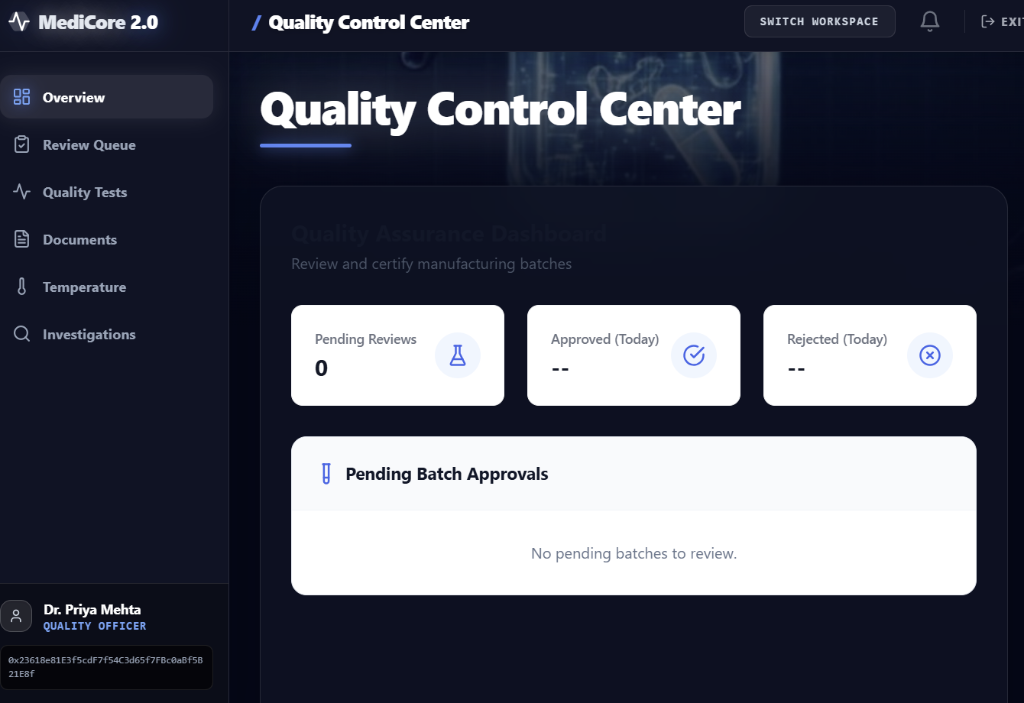
\includegraphics[width=0.88\textwidth]{fig10.png}
\caption{MEDICORE public read-only verification interface showing an authenticated product record, manufacturer and lifecycle information, and cryptographic packaging-seal status. The screenshot demonstrates digital-record verification and is not treated as independent evidence of physical product authenticity.}
\label{fig:public_verify_ui}
\end{figure}

\begin{table}[htbp]
\centering
\caption{MEDICORE prototype dataset used for the current evaluation}
\label{tab:prototype_dataset}
\vspace{0.5em}
\begin{tabularx}{\textwidth}{lcX}
\toprule
\textbf{Item} & \textbf{Count} & \textbf{Description} \\
\midrule
Registered entities & 7 & Manufacturer, wholesaler, retailer, customer, transporter, regulator, and quality officer \\
Operational roles & 8 & Super Admin plus the seven registered participant categories \\
Drug batches & 5 & PARA-2026-001, AMOX-2026-001, INSU-2026-001, VACC-2026-001, and METF-2026-001 \\
Transfer transactions & 8 & Recorded manufacturer, wholesaler, retailer, and customer handoffs \\
Supporting documents & 3 & Manufacturing/quality and laboratory documents represented by the prototype \\
Active recalls & 1 & AMOX-2026-001 \\
Temperature violations & 1 & METF-2026-001, observed at 11.4$^\circ$C against a configured 2--8$^\circ$C range \\
\bottomrule
\end{tabularx}
\end{table}

\subsection{Project-Reported EVM Benchmark Snapshot}
The repository currently reports a local EVM benchmark generated from the implemented experiment tooling. These values are reported as a project benchmark snapshot, not as a claim of production-network performance.

\begin{figure}[htbp]
\centering
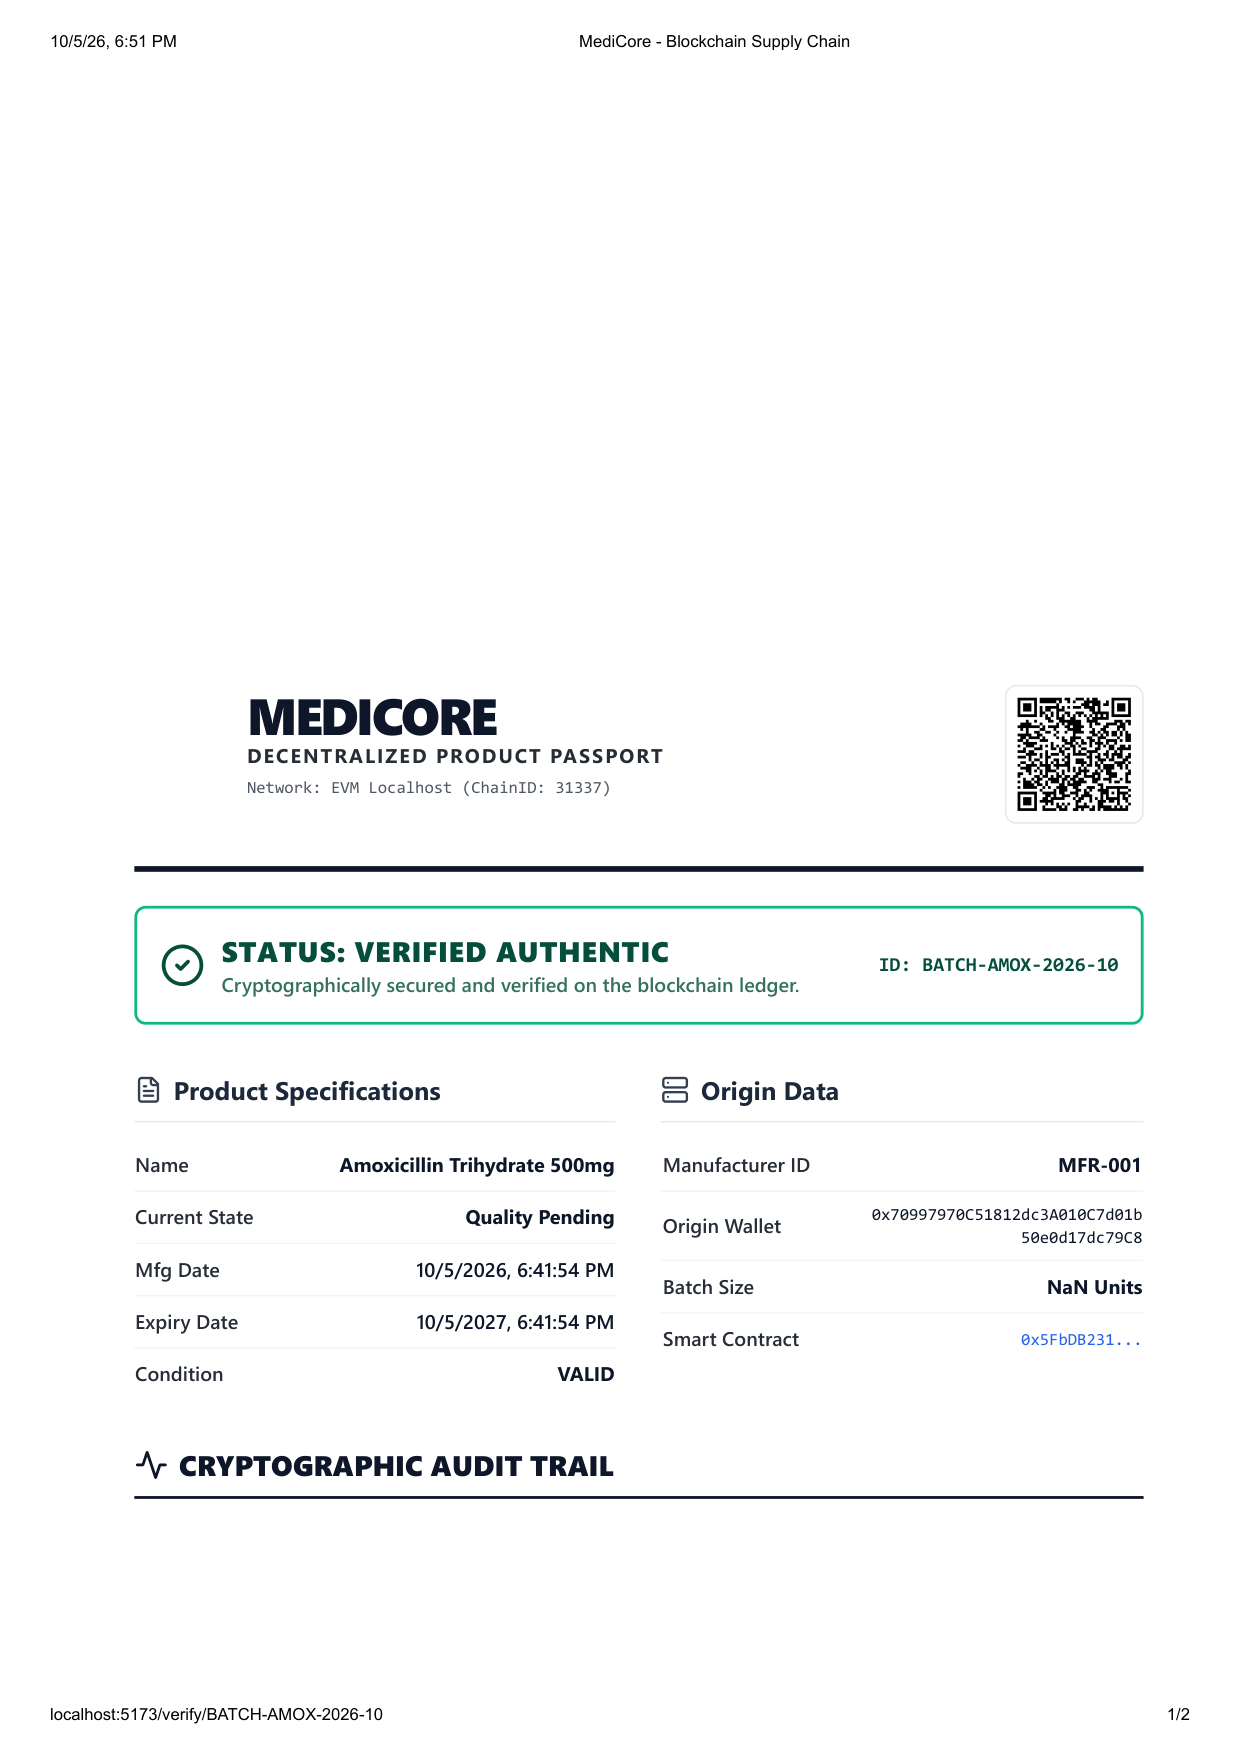
\includegraphics[width=0.75\textwidth]{fig11.png}
\caption{MEDICORE Digital Product Passport generated from the implemented verification workflow. The document contains the batch identity, product specifications, manufacturer identity, smart-contract reference, QR code, and cryptographic audit-trail information.}
\label{fig:passport_ui}
\end{figure}

The benchmark should be interpreted in the context of the local Hardhat/EVM development environment used by the project. In particular, the latency values are not directly comparable with public Ethereum production latency, and the success-rate column does not establish statistical reliability without a documented number of repeated trials. The benchmark is retained because it is generated from the project's implementation and provides a reproducible starting point for further evaluation.

\begin{figure}[htbp]
\centering
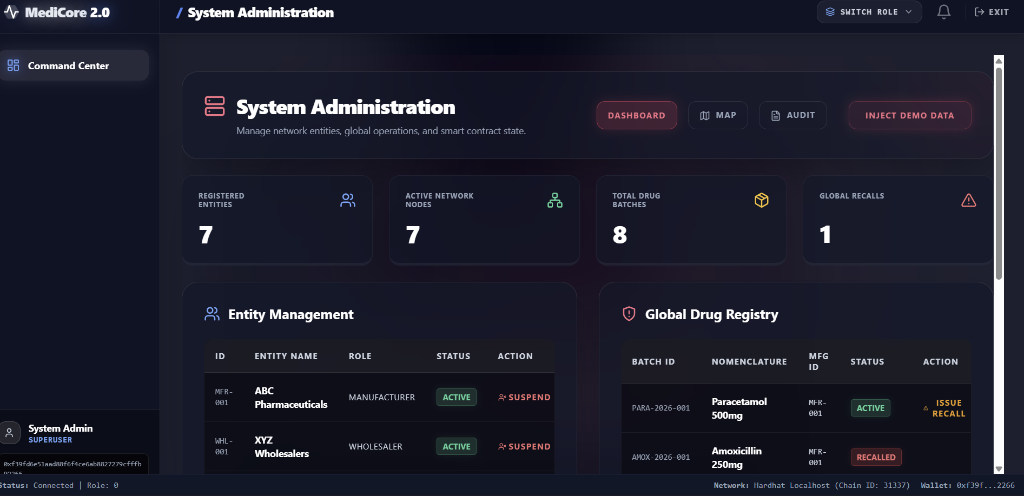
\includegraphics[width=0.88\textwidth]{fig12.png}
\caption{MEDICORE System Administration workspace showing network-entity management and the global drug registry. The administrative interface provides controls for system-level network operations and entity status management.}
\label{fig:admin}
\end{figure}

\begin{table}[htbp]
\centering
\caption{Actual MEDICORE batch and transfer data}
\label{tab:batch_data}
\vspace{0.5em}
\begin{tabularx}{\textwidth}{lrrrl}
\toprule
\textbf{Batch ID} & \textbf{Initial Qty.} & \textbf{Transferred Qty.} & \textbf{Remaining Qty.} & \textbf{Recorded transfer path(s)} \\
\midrule
PARA-2026-001 & 10,000 & 5,550 & 4,450 & MFR$\to$WHL (4,000); WHL$\to$RET (1,500); RET$\to$CUS (50) \\
AMOX-2026-001 & 5,000 & 2,000 & 3,000 & MFR$\to$WHL (2,000) \\
INSU-2026-001 & 2,000 & 500 & 1,500 & MFR$\to$WHL (500) \\
VACC-2026-001 & 50,000 & 13,000 & 37,000 & MFR$\to$WHL (10,000); WHL$\to$RET (3,000) \\
METF-2026-001 & 8,000 & 3,000 & 5,000 & MFR$\to$WHL (3,000) \\
\midrule
\textbf{Total} & \textbf{75,000} & \textbf{24,050} & \textbf{50,950} & Five batches and eight recorded transfers \\
\bottomrule
\end{tabularx}
\end{table}

\subsection{Authorization Experiment}
The role system contains eight operational roles. Authorization testing should use the actual deployed contract roles and the corresponding accounts rather than frontend-selected role labels. For each protected operation, an account with the required role and an account without that role are tested. Authorization accuracy is defined as:
\begin{equation}
AA = \frac{N_{\text{correct}}}{N_{\text{total}}} \times 100
\end{equation}

\begin{table}[htbp]
\centering
\caption{MEDICORE benchmark snapshot reported by the project}
\label{tab:benchmarks_snapshot}
\vspace{0.5em}
\begin{tabular}{lrrr}
\toprule
\textbf{Operation} & \textbf{Average gas} & \textbf{Latency (ms)} & \textbf{Success rate} \\
\midrule
Batch minting & 186,412 & 12.4 & 100\% \\
Quality approval & 52,190 & 9.8 & 100\% \\
Shipment creation & 124,310 & 14.1 & 100\% \\
Cryptographic receipt & 94,820 & 13.5 & 100\% \\
Public QR read & 0 (view) & 11.2 & 100\% \\
\bottomrule
\end{tabular}
\end{table}

The current implementation audit establishes that role-controlled smart-contract operations are implemented, but a complete repeated authorization test set has not yet been recorded. Therefore, no numerical $AA$ value is fabricated in this paper.

\subsection{QR Verification Experiment}
The actual MEDICORE demonstration contains six verification scenarios. Table~\ref{tab:qr_scenarios} maps each scenario to the corresponding prototype condition.

\begin{table}[htbp]
\centering
\caption{Actual MEDICORE QR verification scenarios}
\label{tab:qr_scenarios}
\vspace{0.5em}
\begin{tabularx}{\textwidth}{llX}
\toprule
\textbf{Scenario} & \textbf{Expected status} & \textbf{Prototype condition} \\
\midrule
PARA-2026-001 & \texttt{VERIFIED} & Valid batch with recorded quality approval \\
AMOX-2026-001 & \texttt{WARNING} & Batch has an active recall \\
METF-2026-001 & \texttt{WARNING} & Batch has a recorded temperature violation \\
VACC-2026-001 & \texttt{WARNING} & Demonstration scenario configured for approaching expiry \\
INSU-2026-001 & \texttt{VERIFIED} & Valid batch with cold-chain context \\
Fake/unknown identifier & \texttt{INVALID} & Identifier does not correspond to a valid batch record \\
\bottomrule
\end{tabularx}
\end{table}

For each QR test, the verifier should record the identifier, verification decision, reason, and response time. The current scenarios establish functional coverage; a measured latency distribution requires repeated execution and is therefore reported separately from the existing dataset.

\subsection{Shipment and GPS Monitoring Experiment}
The implemented shipment model associates a shipment with a batch, sender, receiver, transporter, quantity, status, and location information. GPS telemetry records use shipment identifier, latitude, longitude, accuracy, speed, heading, and timestamp fields.

A controlled GPS experiment should include a normal route, a route deviation, a large coordinate jump, and an impossible travel sequence. Route-distance calculations, when required, can use the Haversine distance between two recorded coordinates:
\begin{equation}
d = 2R \arcsin \sqrt{\sin^2\left(\frac{\Delta \phi}{2}\right) + \cos(\phi_1)\cos(\phi_2)\sin^2\left(\frac{\Delta \lambda}{2}\right)}
\end{equation}
where $R$ is the Earth radius and $(\phi, \lambda)$ are latitude and longitude. The current prototype establishes GPS monitoring functionality, but no fabricated route-deviation percentage is reported without a logged ground-truth experiment.

\subsection{Cold-Chain Experiment}
The current dataset contains one explicit temperature-violation scenario for METF-2026-001. The configured acceptable interval is 2--8$^\circ$C and the observed value is 11.4$^\circ$C. The deviation above the configured maximum is therefore 3.4$^\circ$C.

The violation indicator is defined as:
\begin{equation}
V_T = \begin{cases} 1, & T < T_{\min} \text{ or } T > T_{\max} \\ 0, & T_{\min} \le T \le T_{\max} \end{cases}
\end{equation}
For METF-2026-001, $V_T = 1$ because $11.4 > 8$. The result indicates a condition requiring investigation or warning; it does not by itself prove physical drug damage or counterfeit status. Continuous hardware-based sensing remains future work for the current prototype.

\subsection{Recall Propagation Experiment}
AMOX-2026-001 is the current active-recall scenario. The prototype records the recall workflow and uses recall state during verification so that the affected batch is not presented as normally verified.

Recall propagation can be measured across the interfaces that are expected to reflect the recall state:
\begin{equation}
RP = \frac{N_{\text{affected interfaces correctly updated}}}{N_{\text{expected interfaces}}} \times 100
\end{equation}
For the current paper, the affected interfaces are batch verification, shipment verification, and regulator visibility. A numerical propagation percentage should be inserted only after the controlled test has recorded all three observations.

\subsection{Traceability Completeness}
Traceability is evaluated by comparing the lifecycle events expected for a selected batch with the events actually recorded in the prototype:
\begin{equation}
TC = \frac{N_{\text{observed lifecycle events}}}{N_{\text{expected lifecycle events}}} \times 100
\end{equation}
The denominator must be defined before the experiment for the selected workflow; it must not be changed after observing the results. Because the present source data do not contain a separately logged expected-event matrix, a final numerical $TC$ value is not inserted here.

\begin{figure}[htbp]
\centering
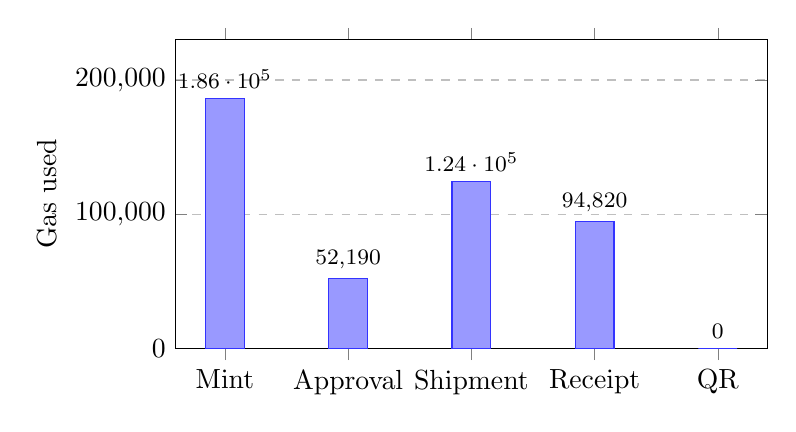
\begin{tikzpicture}
\begin{axis}[
    ybar,
    bar width=14pt,
    width=0.75\textwidth,
    height=5.5cm,
    ylabel={Gas used},
    symbolic x coords={Mint, Approval, Shipment, Receipt, QR},
    xtick=data,
    nodes near coords,
    nodes near coords align={vertical},
    every node near coord/.append style={font=\footnotesize},
    ymin=0, ymax=230000,
    yticklabel style={/pgf/number format/fixed},
    scaled y ticks=false,
    ymajorgrids=true,
    grid style=dashed
]
\addplot[fill=blue!40, draw=blue!80] coordinates {
    (Mint, 186412)
    (Approval, 52190)
    (Shipment, 124310)
    (Receipt, 94820)
    (QR, 0)
};
\end{axis}
\end{tikzpicture}
\caption{Reported local-EVM gas consumption for the five benchmark operations in the current MEDICORE README. Public QR verification is a read-only call and therefore consumes zero transaction gas.}
\label{fig:gas_barchart}
\end{figure}

\subsection{Blockchain and API Performance Experiment}
Performance measurements are collected from the actual MEDICORE implementation for operations such as batch creation, quality approval, transfer, shipment creation, shipment receipt, recall operations, entity suspension/reinstatement, QR verification, API requests, GPS ingestion, and temperature ingestion.

For a blockchain transaction, confirmation latency is:
\begin{equation}
L_{\text{tx}} = T_{\text{confirmation}} - T_{\text{submission}}
\end{equation}
For API or verification operations, the corresponding request-to-response interval is recorded. Gas usage is read from the actual transaction receipt rather than estimated from a literature benchmark. Each operation should be repeated under the same local Hardhat/network configuration, and mean, median, minimum, maximum, and standard deviation should be reported. The current repository already reports a benchmark snapshot for five lifecycle operations (Table~\ref{tab:benchmarks_snapshot}); additional repeated measurements are required before broader statistical claims are made.

\section{Results and Evaluation}
The results are divided into dataset-derived results and measurements that require controlled repeated execution. This separation prevents prototype inventory data from being presented as a benchmark dataset.

\subsection{Dataset-Derived Results}
Table~\ref{tab:dataset_results} summarizes the directly supported results from the current MEDICORE dataset.

\begin{table}[htbp]
\centering
\caption{Results directly derived from the current MEDICORE prototype dataset}
\label{tab:dataset_results}
\vspace{0.5em}
\begin{tabularx}{\textwidth}{lrX}
\toprule
\textbf{Metric} & \textbf{Value} & \textbf{Interpretation} \\
\midrule
Registered entities & 7 & Seven participant entities are represented in the current demonstration \\
Operational roles & 8 & Includes Super Admin and seven supply-chain participant categories \\
Drug batches & 5 & Five named pharmaceutical batches are represented \\
Transfer transactions & 8 & Eight transfer records are represented \\
Initial batch quantity & 75,000 & Sum of the five initial batch quantities \\
Transferred quantity & 24,050 & Sum of the recorded outgoing transfers \\
Remaining quantity & 50,950 & Sum of the derived remaining quantities \\
Quantity-conservation checks & 5/5 (100\%) & All five batch equations balance \\
Active recalls & 1 & AMOX-2026-001 is the active recall scenario \\
Temperature violations & 1 & METF-2026-001 at 11.4$^\circ$C against 2--8$^\circ$C \\
Supporting documents & 3 & Documents represented in the prototype demonstration \\
\bottomrule
\end{tabularx}
\end{table}

\subsection{Batch-Level Quantity Results}
The batch-level results are given in Table~\ref{tab:batch_quantity_results}. These values are calculated from the actual transfer records rather than from synthetic workload generation.

\begin{table}[htbp]
\centering
\caption{Batch-level quantity conservation results}
\label{tab:batch_quantity_results}
\vspace{0.5em}
\begin{tabular}{lrrrr}
\toprule
\textbf{Batch} & \textbf{Initial} & \textbf{Transferred} & \textbf{Remaining} & \textbf{Utilization} \\
\midrule
PARA-2026-001 & 10,000 & 5,550 & 4,450 & 55.5\% \\
AMOX-2026-001 & 5,000 & 2,000 & 3,000 & 40.0\% \\
INSU-2026-001 & 2,000 & 500 & 1,500 & 25.0\% \\
VACC-2026-001 & 50,000 & 13,000 & 37,000 & 26.0\% \\
METF-2026-001 & 8,000 & 3,000 & 5,000 & 37.5\% \\
\bottomrule
\end{tabular}
\end{table}

\subsection{QR Verification Results}
The current verification scenarios provide coverage of valid, recalled, temperature-warning, approaching-expiry, cold-chain, and invalid-identifier conditions. The intended outputs are shown in Table~\ref{tab:qr_results}.

\begin{table}[htbp]
\centering
\caption{MEDICORE QR verification result scenarios}
\label{tab:qr_results}
\vspace{0.5em}
\begin{tabularx}{\textwidth}{lll}
\toprule
\textbf{Batch/Case} & \textbf{Result} & \textbf{Reason} \\
\midrule
PARA-2026-001 & \texttt{VERIFIED} & Valid blockchain-backed batch and approved quality state \\
AMOX-2026-001 & \texttt{WARNING} & Active recall state \\
METF-2026-001 & \texttt{WARNING} & Recorded temperature excursion \\
VACC-2026-001 & \texttt{WARNING} & Approaching-expiry demonstration condition \\
INSU-2026-001 & \texttt{VERIFIED} & Valid batch with cold-chain context \\
Unknown/fake identifier & \texttt{INVALID} & No corresponding valid batch record \\
\bottomrule
\end{tabularx}
\end{table}

These results demonstrate the intended distinction between normal verification and warning conditions. In particular, a warning caused by a recall or environmental incident is not equivalent to a claim that the medicine is physically counterfeit.

\subsection{Cold-Chain Result}
The METF-2026-001 scenario provides a concrete controlled condition: the configured interval is 2--8$^\circ$C and the observed value is 11.4$^\circ$C. The system therefore evaluates the temperature as a violation ($V_T = 1$) and associates the batch with a warning/investigation condition. The result is a digital monitoring event and should not be interpreted as proof of product degradation without pharmaceutical quality testing.

\subsection{Recall Result}
AMOX-2026-001 is the active recall case in the current prototype. The recall workflow records the affected batch and uses the recall state during verification. A final recall-propagation percentage is intentionally not reported until the batch-verification, shipment-verification, and regulator-view observations have been captured as a controlled test.

\subsection{Reported Blockchain Performance and Automated Tests}
The project README reports a local EVM benchmark covering batch minting, quality approval, shipment creation, cryptographic receipt, and public QR reading. The reported average gas values range from 52,190 gas for quality approval to 186,412 gas for batch minting, while the reported latency values range from 9.8 to 14.1 ms for the state-changing operations and 11.2 ms for public QR reading. Public QR verification is implemented as a read-only operation and therefore reports zero transaction gas in the benchmark.

The repository also reports six automated contract tests passing in approximately one second. The test cases cover entity registration, batch manufacture, quality approval, shipment creation with quantity conservation, shipment receipt, and suspension of an entity followed by action blocking. These tests provide functional evidence for core contract workflows, while not constituting a complete security audit or production-scale evaluation.

\subsection{Authorization and Performance Results}
The prototype implements role-controlled operations and the required performance-measurement hooks, but the current dataset does not contain a sufficiently complete repeated test log to support a numerical authorization accuracy or performance benchmark. Therefore, the following values must be populated from actual execution logs rather than estimated values:

\begin{table}[htbp]
\centering
\caption{Measurements to be collected from controlled MEDICORE executions}
\label{tab:measurements}
\vspace{0.5em}
\begin{tabularx}{\textwidth}{lX}
\toprule
\textbf{Measurement} & \textbf{Required experimental record} \\
\midrule
Authorization accuracy & Correct versus incorrect decisions across authorized and unauthorized role-operation pairs \\
Traceability completeness & Observed versus pre-defined expected lifecycle events \\
Recall propagation & Correctly updated interfaces divided by expected interfaces \\
Transaction latency & Submission-to-confirmation time from blockchain receipts/logs \\
Gas consumption & Actual gas used for each smart-contract operation \\
QR latency & Time from QR verification request to returned status \\
GPS ingestion latency & Time from telemetry submission to persisted/visible record \\
Temperature ingestion latency & Time from observation submission to incident evaluation \\
Anomaly detection rate & Detected known anomalies divided by known injected anomalies \\
\bottomrule
\end{tabularx}
\end{table}

\section{Security and Threat Analysis}

\subsection{Unauthorized Operations}
Role-based smart-contract modifiers prevent unauthorized participants from executing protected operations.

\subsection{Quantity Manipulation}
Quantity conservation rules restrict transfers to the available quantity recorded for the batch.

\subsection{Replay of Shipment Receipt}
A shipment that has already been received should not be receivable again. The shipment state is therefore checked before receipt.

\subsection{Suspended Entity Operations}
Administrative suspension changes the entity state and prevents restricted operations according to the smart-contract authorization rules.

\subsection{Data Tampering}
Blockchain records provide tamper-evident transaction history. However, blockchain integrity does not guarantee that the original off-chain information was truthful.

\subsection{Physical Authenticity}
A critical limitation is that digital verification does not automatically establish physical product authenticity. A compromised physical label or QR code could potentially be associated with a legitimate digital record. Consequently, MEDICORE should be considered a traceability and verification framework rather than a complete physical anti-counterfeiting guarantee.

\subsection{Off-Chain Data}
GPS, temperature, and document information depend on off-chain infrastructure. Therefore, the integrity and security of sensors, APIs, databases, and storage services remain important components of the overall security model.

\section{Discussion}
MEDICORE demonstrates an integrated approach to pharmaceutical supply-chain traceability in which blockchain is used selectively for information requiring shared integrity and authorization, while operational telemetry is maintained off-chain.

A blockchain-only design would be inefficient for continuously generated GPS and temperature observations. The hybrid design therefore separates high-integrity transactional information from high-volume operational data.

The permanent entity identity mechanism additionally provides a stable reference connecting organizational information, facilities, licenses, shipments, batches, and audit records. This is useful because wallet addresses are technical credentials rather than persistent organizational identities.

The quantity-conservation mechanism addresses an important supply-chain consistency requirement. While blockchain cannot determine whether a physical shipment contains the declared quantity, it can prevent inconsistent digital transfer operations within the recorded system.

The QR mechanism improves accessibility by allowing users to access product records without requiring direct blockchain interaction. However, the distinction between digital record verification and physical authentication remains important.

The anomaly-monitoring layer provides an additional intelligence component. Route deviations, temperature excursions, suspicious QR scans, and quantity inconsistencies can be converted into investigation signals. Such signals should support human investigation rather than automatically establish fraud or unlawful activity.

\section{Limitations}
The current MEDICORE prototype has several limitations:
\begin{enumerate}
    \item Continuous physical IoT sensing may not yet be available in the prototype environment. Temperature experiments may therefore use simulated telemetry.
    \item The current implementation associates Certificate of Analysis evidence with IPFS-oriented cryptographic references, but production-grade decentralized storage and long-term pinning should be validated independently before deployment.
    \item The customer-facing integration may be less complete than the internal supply-chain workflows.
    \item The backend requires stronger authentication mechanisms before production deployment. In particular, frontend-provided identity information should not be treated as sufficient authorization for sensitive backend operations.
    \item Large-scale performance under production pharmaceutical supply-chain workloads has not been evaluated.
    \item The prototype does not guarantee physical authenticity merely because a blockchain record is valid.
    \item The current cold-chain component is a simulator rather than a deployed fleet of calibrated physical sensors.
    \item Machine-learning-based anomaly detection requires sufficiently large and representative operational datasets. The current Sentinel layer provides operational/rule-based anomaly indicators, while large-scale learned models remain future work.
\end{enumerate}

\section{Future Work}
Future development will focus on the following areas:
\begin{enumerate}
    \item Integration of ESP32-based temperature sensors and industrial IoT devices.
    \item Continuous cold-chain telemetry collection.
    \item Secure GPS integration for logistics providers.
    \item Production-grade IPFS or equivalent decentralized document storage.
    \item Wallet-signature-based backend authentication.
    \item Mobile applications for manufacturers, logistics providers, pharmacies, and consumers.
    \item Machine-learning models for supply-chain anomaly detection.
    \item Predictive risk analysis using historical shipment and temperature data.
    \item Interoperability with pharmaceutical regulatory systems.
    \item Scalable blockchain deployment using appropriate production infrastructure.
    \item Privacy-preserving verification mechanisms.
    \item Formal smart-contract verification.
\end{enumerate}

\section{Conclusion}
This paper presented MEDICORE, a hybrid blockchain-based framework for pharmaceutical supply-chain traceability, verification, monitoring, and anomaly identification. The framework integrates role-based smart contracts, permanent entity identities, pharmaceutical batch records, quantity conservation, shipment verification, digital product passports, QR-based verification, GPS monitoring, cold-chain monitoring, recall management, and administrative audit mechanisms.

The proposed architecture separates blockchain-critical records from high-volume operational information, allowing blockchain to provide shared integrity and authorization while databases and monitoring services manage continuous telemetry.

The experimental methodology provides a reproducible basis for evaluating authorization, quantity conservation, traceability, QR verification, anomaly monitoring, recall propagation, and operational performance. The current project benchmark reports 186,412 gas for batch minting, 52,190 gas for quality approval, 124,310 gas for shipment creation, 94,820 gas for cryptographic receipt, and zero transaction gas for public QR reads, with reported latencies between 9.8 and 14.1 ms for the state-changing operations. These measurements are explicitly interpreted as local development-environment results rather than production-network guarantees.

MEDICORE does not claim that blockchain alone eliminates counterfeit medicines or illegal diversion. Instead, it provides a digital infrastructure intended to improve traceability, visibility, controlled information sharing, and detection of supply-chain events requiring investigation. The framework demonstrates the potential of combining blockchain with intelligent monitoring mechanisms to create a more auditable and connected pharmaceutical supply chain.

\section*{Declarations}

\subsection*{Funding}
No external funding was received for this research.

\subsection*{Competing Interests}
The authors declare that they have no competing interests.

\subsection*{Ethics Approval and Consent to Participate}
This research involves a software prototype and does not involve human participants, human samples, or animal experiments.

\subsection*{Consent for Publication}
Not applicable.

\subsection*{Data Availability}
The experimental data generated from the MEDICORE prototype will be made available with the research materials where permitted. No private credentials or sensitive personal information are included.

\subsection*{Materials Availability}
The software prototype and configuration required for reproducibility can be provided subject to institutional and project requirements.

\subsection*{Code Availability}
The source code and reproducibility materials are maintained in the public MEDICORE repository at \url{https://github.com/bhumiadi23/MEDICORE}. The repository includes the blockchain contract, deployment and seed scripts, automated tests, backend, frontend, research scripts, benchmark outputs, and the research-paper directory.

\subsection*{Author Contributions}
Aditya Kumar Roy contributed to system architecture, blockchain integration, frontend development, experimentation, and manuscript preparation. Krishna Das contributed to blockchain implementation, testing, backend integration, documentation, and system evaluation. Both authors reviewed and approved the manuscript.

\subsection*{Acknowledgements}
The authors would like to thank the Department of Computer Science and Engineering, C. V. Raman Global University, Bhubaneswar, Odisha, for providing the academic environment and resources required to develop this project.

\begin{thebibliography}{99}

\bibitem{who2024substandard}
World Health Organization. Substandard and falsified medical products. WHO Fact Sheet, 2024.

\bibitem{who2017substandard}
World Health Organization. 1 in 10 medical products in developing countries is substandard or falsified. WHO, 2017.

\bibitem{liu2021blockchain}
Liu X, Barenji AV, Li Z, Montreuil B, Huang GQ. Blockchain-based smart tracking and tracing platform for drug supply chain. \textit{Computers \& Industrial Engineering}. 2021;161:107669.

\bibitem{hosseini2021blockchain}
Hosseini Bamakan SM, Ghasemzadeh Moghaddam S, Dehghan Manshadi S. Blockchain-enabled pharmaceutical cold chain: Applications, key challenges, and future trends. \textit{Journal of Cleaner Production}. 2021;302:127021.

\bibitem{nagasudha2024trackchain}
Naga Sudha CM, Nayahi JVJ. TrackChain: Hyperledger based pharmaceutical supply chain -- Resource utilization perspective. \textit{Heliyon}. 2024;10:e23250.

\bibitem{akram2024blockchain}
Akram W, Joshi R, Haider T, et al. Blockchain technology: A potential tool for the management of pharma supply chain. \textit{Research in Social and Administrative Pharmacy}. 2024;20(6):156--164.

\bibitem{henrichs2025quantum}
Henrichs E, Boller ML, Stolz J, Krupitzer C. Quantum of Trust: Overview of Blockchain Technology for Product Authentication in Food and Pharmaceutical Supply Chains. \textit{Trends in Food Science \& Technology}. 2025;157:104892.

\bibitem{nakamoto2008bitcoin}
Nakamoto S. Bitcoin: A Peer-to-Peer Electronic Cash System. Technical report. 2008.

\bibitem{szabo1997formalizing}
Szabo N. Formalizing and Securing Relationships on Public Networks. \textit{First Monday}. 1997;2(9).

\bibitem{crosby2016blockchain}
Crosby M, Pattanayak P, Verma S, Kalyanaraman V. Blockchain technology: Beyond bitcoin. \textit{Applied Innovation Review}. 2016;2:6--19.

\bibitem{casino2019systematic}
Casino F, Dasaklis TK, Patsakis C. A systematic literature review of blockchain-based applications: Current status, classification and open issues. \textit{Telematics and Informatics}. 2019;36:55--81.

\bibitem{kamilaris2019rise}
Kamilaris A, Fonts A, Prenafeta-Boldu FX. The rise of blockchain technology in agriculture and food supply chains. \textit{Trends in Food Science \& Technology}. 2019;91:640--652.

\bibitem{saberi2019blockchain}
Saberi S, Kouhizadeh M, Sarkis J, Shen L. Blockchain technology and its relationships to sustainable supply chain management. \textit{International Journal of Production Research}. 2019;57(7):2117--2135.

\bibitem{queiroz2020blockchain}
Queiroz MM, Telles R, Bonilla SH. Blockchain and supply chain management integration: A systematic review of the literature. \textit{Supply Chain Management: An International Journal}. 2020;25(2):241--254.

\bibitem{wang2019understanding}
Wang Y, Han JH, Beynon-Davies P. Understanding blockchain technology for future supply chains: A systematic literature review and research agenda. \textit{Supply Chain Management: An International Journal}. 2019;24(1):62--84.

\bibitem{yadav2022blockchain}
Yadav AK, Shweta, Kumar D. Blockchain technology and vaccine supply chain: Exploration and analysis of the adoption barriers in the Indian context. \textit{International Journal of Production Economics}. 2022.

\bibitem{antal2018blockchain}
Antal C, Cioara T, Anghel I, Antal M, Salomie I. Blockchain based decentralized system for cold chain management. \textit{International Conference on Automation, Quality and Testing, Robotics}. 2018.

\bibitem{mutambik2026blockchain}
Mutambik I. A Blockchain--IoT--ML Framework for Sustainable Vaccine Cold Chain Management in Pharmaceutical Supply Chains. \textit{Systems}. 2026;14(5):467.

\bibitem{securitythreats2026}
Security Threats in Blockchain-IoT Pharmaceutical Cold Chain Management Systems: A Survey. \textit{IEEE ICITSIF}. 2026. doi:10.1109/ICITSIF69060.2026.11608768.

\bibitem{gs12024epcis}
GS1. EPCIS and Core Business Vocabulary. GS1 Standard. 2024.

\bibitem{gs12024healthcare}
GS1. Healthcare Traceability and GS1 Standards. GS1 Healthcare. 2024.

\bibitem{gs12017global}
GS1. GS1 Global Traceability Standard. GS1 Standard. 2017.

\bibitem{dutta2026blockchain}
Dutta D, Priya G. Blockchain-based solution for secure and transparent pharmaceutical supply chain management using drugledger. \textit{Scientific Reports}. 2026;16:28622.

\bibitem{hasan2026blockchain}
Hasan MN, Datta S, Namasudra S. Blockchain-based pharmaceutical supply chain: a scalable and transparent model for drug traceability. \textit{Peer-to-Peer Networking and Applications}. 2026;19:139.

\bibitem{rajak2026scalable}
Rajak DK, Khanal B, Ansari MSA. Scalable blockchain-based solution for drug tracking in pharmaceutical supply chain. \textit{Computers \& Industrial Engineering}. 2026;211:111655.

\bibitem{drugtrace2026}
DrugTrace: Leveraging blockchain and IoT for anti-counterfeit drug traceability. \textit{SoftwareX}. 2026;34:102694.

\bibitem{zk2026privacy}
Zero-Knowledge Proof-Based Privacy-Preserving Pharmaceutical Traceability and Recall Using Blockchain. \textit{Blockchains}. 2026;4(2):5.

\bibitem{devi2025blockchain}
Devi PY, Sriramya P, Khilar R. Blockchain reputation-based consensus mechanism for distributed medical supply chain drug traceability with pyramidal ShuffleNet. \textit{Discover Computing}. 2025;28:24.

\bibitem{siyal2026traceability}
Siyal F, Guzzo A, Alkhabbas F, et al. From traceability to intelligence: a review of blockchain, IoT, and AI for transparent supply chains. \textit{Cluster Computing}. 2026;29:325.

\end{thebibliography}

\end{document}
